\documentclass{article}

\usepackage{amsmath}
\usepackage{amsfonts}
\usepackage{amssymb}
\usepackage[inference]{semantic}
\usepackage{mathtools}

\title{Type and Programming Languages}
\author{Hoblovski}

\newcommand{\nset}{\mathbb{N}}
\newcommand{\rset}{\mathbb{R}}
\newcommand{\ite}[3]{\text{if}\; #1 \; \text{then}\; #2 \; \text{else}\; #3}
\newcommand{\lett}[3]{\text{let}\; #1\, =\, #2 \;\text{in}\; #3}
\newcommand{\lam}[2]{\lambda #1 .\;#2}
\newcommand{\lamt}[3]{\lambda #1: #2 .\;#3}
\newcommand{\lamk}[3]{\lambda #1 :: #2 .\;#3}
\newcommand{\app}[2]{#1\, #2}
\newcommand{\appp}[2]{\left(#1\, #2\right)}
\newcommand{\tapp}[2]{#1\, \left[#2\right]}
\newcommand{\typjud}[2]{\Gamma \vdash #1: #2}
\newcommand{\typjudp}[2]{\Gamma \vdash \left(#1\right): #2}
\newcommand{\typjudr}[2]{\Gamma,\; \Sigma \vdash #1: #2}
\newcommand{\typjudrp}[2]{\Gamma, \; \Sigma \vdash \left(#1\right): #2}
\newcommand{\typjudc}[3]{\Gamma \vdash #1: #2 \;| #3}
\newcommand{\typjudcp}[3]{\Gamma \vdash \left(#1\right): #2 \;| #3}
\newcommand{\mtrue}{\mathrm{true}}
\newcommand{\mfalse}{\mathrm{false}}
\newcommand{\mref}{\mathrm{ref}\, }
\newcommand{\mtop}{\mathrm{top}}
\newcommand{\mbot}{\mathrm{bot}}
\newcommand{\mRef}{\mathrm{Ref}\, }
\newcommand{\munit}{\text{unit}}
\newcommand{\dom}{\mathrm{dom}}
\newcommand{\uquant}[2]{\forall #1 \, .\; #2}
\newcommand{\equant}[2]{\exists #1 \, .\; #2}
\newcommand{\epack}[2]{#1 \,\mathrm{as}\; #2}
\newcommand{\elet}[4]{\text{let}\; \{#1, #2\}\, =\, #3 \;\text{in}\; #4}

% Setting all equations left justified
%
% \documentclass[fleqn]{article}
% \usepackage{amsmath}
% \setlength{\mathindent}{2em}

\begin{document}
\maketitle
\tableofcontents



\section{Ch3: Untyped Arithmetic Expressions}
\subsection{Concepts}
  \begin{itemize}
    \item Term: Definable by either induction, inference rules, or generational ($\mathcal{S} = \cup_{i \in \nset} \mathcal{S}_i$)
    \item Metavariable: Placeholder that ranges over certain sorts of entities in the object language. Different from ``variable'' in the object language.
    \item Value: terms evaluate to values. Values can't be further evaluated or reduced. In chapter 3 terms do not include values.
    \item Inference rule, axiom, proper rule.
    \item Rule schema: inference rules whose premise or conclusive might include metavariables.
    \item{} [Structural] operational semantics: semantics through definition of an abstract machine.
      To describe the machine, the following components are needed: 1) a set of states,
      2) a function that specifies the state transition when the term is simplified a step.
      The semantics of a term is the halting state of the machine after simplifying the term.
    \item{} Natural [operational] semantics: $t\Downarrow v$ denote that term $t$ evaluates to final value $v$.
    \item Denotational semantics: meaning of a term is represented by some mathematical object,
      e.g. a number or a function. A denotational semantics consists of a \emph{semantic domain}, and a
      \emph{interpretation function} mapping terms into elements in the semantic domain.
    \item Axiomatic semantics: the semantics laws themselves, either operational or denotational,
      become the definition of the language. The meaning of a term is what we can prove about it.
    \item Normal form terms: terms which no reduction rules apply to.
      There're theorems: 1) values are always in normal forms; 2) normal form terms that aren't runtime errors are values.
    \item Reduction relation and evaluation relation.
    \item Stuck: a normal form that's not a value. Models runtime error in real programs.
  \end{itemize}

\subsection{Takeaways}
  In operational semantics, $t \to t'$ reads like ``in a single step $t$ reduces to $t'$''

  An \emph{instance} of an inference rule is obtained by consistently replacing
    metavariables by terms in the rule's premises and conclusion.

  The derivation tree on page 36 does not state an ``evaluation derivation'' but rather a ``reduction derivation'',
  i.e. the conclusion it derives is a valid single-step reduction.



\section{Ch5: Untyped Lambda-Calculus}
\subsection{Elements}
  \label{untyp}
  Only condider pure untyped lambda-calculus without based types.

\paragraph{Terms}
  \begin{align*}
    t \quad ::= \quad & x \tag{variable} \\
      & \lam{x}{t} \tag{abstraction} \\
      & \app{t}{t} \tag{application}\\
  \end{align*}

\paragraph{Values}
  \begin{align*}
    v \quad ::= \quad & \lam{x}{t} \tag{abstraction} \\
  \end{align*}

\paragraph{Semantics}
  \begin{align*}
    & \inference{t_1 \to t_1'}{\app{t_1}{t_2} \to \app{t_1'}{t_2}}  \tag{E-APP1} \\
    & \inference{t_2 \to t_2'}{\app{v}{t_2} \to \app{v}{t_2'}}  \tag{E-APP2} \\
    & (\lam{x}{t}) v \to [x\mapsto v]\, t \tag{E-APPABS} \\
  \end{align*}

\subsection{Concepts}
  \begin{itemize}
    \item Terms: only 3 types: 1) atom variables, 2) (function) abstraction, 3) (function) application.
    \item Lambda terms could be written in abstract hierarchical form.
    \item Bound: $x$ in bound in an term if the term is (possible indirectly) enclosed in an abstraction $\lambda x\, .\, \ldots$
      Intuitively the name of bound variables do not matter.
    \item Free variables are not bound, like $x$ in $\lambda y\, .\, x y$.
    \item A term without free variables is called closed, a.k.a. combinator. Note by definition terms are not necessarily closed.
% t: metavariable ranging over terms;  x: metavariable ranging over variables.
    \item Untyped lambda calculus is Turing complete.
  \end{itemize}

\subsection{Semantics}
  \begin{itemize}
    \item $\beta$-reduction: semantics of application $(\lambda x\, t_1) t_2 \rightarrow [x\mapsto t_2] t_1$.
    \item Evaluation strategies: full beta reduction, normal, call-by-name, call-by-value.
      Determines order of reductions and what reductions are allowed.
    \item \emph{Full beta reduction} means any \emph{redex} (reducible expression) can be reduced at any time.
    \item \emph{Normal order} means always reduce the leftmost i.e. outermost redex.
    \item \emph{Call by name} is more restrictive because it disallows reductions inside abstractions.
    \item \emph{Call by value} require that when reducing an abstraction its rhs (operand) must be a value.
  \end{itemize}

\subsection{Church representation}
  \begin{itemize}
    \item Example: define \texttt{true} as $\lambda t\, .\, \lambda f\, .\, t$, and \texttt{false} as $\lambda t\, .\, \lambda f\, .\, f$.
      The technique of defining primitives with pure lambda terms is called church numerals/booleans/\ldots
    \item Divergent combinator: $(\lambda x \,.\, x \, x) (\lambda x \, .\, x \, x)$. Reducing it gives itself.
    \item Call-by-value Y combinator: a.k.a. Z combinator, fixed-point combinator. It's a derivation of the divergent combinator. \[
        \lambda f\, .\, \Big (\lambda x\, .\, f (\lambda y \, .\, x\, x\, y)\Big ) \Big (\lambda x\, .\, f (\lambda y \, .\, x\, x\, y)\Big )\]
    \item E.g. $\text{fact} = \mathcal{Y} g, \, \text{where}\, g = \lambda f\, .\, \lambda n\, .\, \text{if}\, n = 0 \, \text{then}\, 1 \, \text{else}\, n \times f(n-1)$
  \end{itemize}

\subsection{Substitution}
  Substitution meets many subtleties.
  For example $[x \mapsto y](\lambda x\, .\, x)$ shouldn't become $\lambda x\, .\, y$,
  and $[y \mapsto x](\lambda x\, .\, y)$ shouldn't become $\lambda x\, .\, x$.

  Terms only differing in names of bounded variables are interchangeable in all contexts.
  The process of consistently renaming bound variables is called ``\emph{alpha conversion}''.
  Note that not all substitutions are legal.

\subsection{Operational semantics}
  Defined by the evaluation which by careful use of metavariables determines the order of evaluation.

  Intuition is that \begin{itemize}
    \item Any term that is not a value must be some application $t_1 t_2$.
    \item If $t_1$ is not a value, we try to evaluate it first.\[
      \inference{t_1 \to t_1'}{t_1\,  t_2 \to t_1'\,  t_2}\]
    \item If the operator is a value, we try to evaluate the operand \[
      \inference{t \to t'}{v\,  t \to v\,  t'}\]
    \item Finally there comes application itself \[
      (\lambda x\, .\, t_1)\,  v_2 \to [x\mapsto v_2] t_1\]
  \end{itemize}



\section{Ch8: Typed Arithmetic Expressions}
\subsection{Concepts}
  \begin{itemize}
    \item Evaluating a term either yields in a value or get stuck (erroneous term).
    \item Metavariables range over values, terms and now types.
    \item Types are program properties available without running the program.
    \item \emph{Typing relation}: in the form $t \, :\, T$, also written as $t \in T$,
      where $t$ and $T$ are metavariables ranging over terms and types.
    \item Typing relation is defined as the smallest binary relation satisfying all instances of typing rules (schemas).
    \item $t$ is \emph{well-typed} if there exists $T$ such that $t\, :\, T$.
    \item Typing derivation is a hierarchical structure demonstrating that for some $t$ it holds that $t\, :\, T$.
    \item For the simple types in Ch8, well-typed terms have only one unique type.
    \item Values have canonical forms e.g. the canonical form of boolean values consists of only $\mtrue$ and $\mfalse$.
  \end{itemize}

\subsection{Type Soundness}
  \begin{itemize}
    \item \emph{Safety / soundness} means well-typed terms must reduce to a value.
    \item Prove soundness by induction: progress (well-typed normal terms are reducible),
      and preservation (the reduction result is either a value or another well-typed normal term).
  \end{itemize}



\section{Ch9: Simply Typed Lambda-Calculus}
\subsection{Elements}
  \label{simtyp}
  On top of~\ref{untyp}, see page~\pageref{untyp}.
  Often written as abbreviation STLC or $\lambda_{\to}$.

\paragraph{Types}
  \begin{align*}
    T \quad::= \quad & T \to T \tag{function type} \\
  \end{align*}

\paragraph{Contexts}
  \begin{align*}
    \Gamma \quad ::= \quad & \emptyset \tag{empty} \\
      & \Gamma, \, x : T \tag{variable binding} \\
  \end{align*}

\paragraph{Typing}
  \begin{align*}
    & \inference{x:T \in \Gamma}{\typjud{x}{T}} \tag{T-VAR} \\
    & \inference
      {\Gamma, x: T_1 \vdash t_2: T_2}
      {\typjudp{\lamt{x}{T_1}{t_2}}{T_1 \to T_2}}
      \tag{T-ABS} \\
    & \inference{\typjud{t_1}{T_1 \to T_2}, & \typjud{t_2}{T_1}}{\typjud{\app{t_1}{t_2}}{T_2}} \tag{T-APP} \\
  \end{align*}

\subsection{Examples}
  Assuming ordinary addition $\inference{\typjud{x}{\nset},& \typjud{y}{\nset}}{\typjud{x+y}{\nset}}$, derive that \[
    \vdash \left(\lamt{x}{\nset}{\lamt{y}{\nset}{x+y}}\right)\quad:\quad \nset\to\nset\to\nset\]

  Proof:
  \[
    \inference[T-ABS]
    {\inference[T-ABS]
      {\inference[T-ADD]
        {
          x:\nset, \;y:\nset\vdash x: \nset,&
          x:\nset, \;y:\nset\vdash y: \nset
        }
        {x:\nset, \;y:\nset\vdash x+y: \nset}
      }
      {x:\nset \vdash (\lamt{y}{\nset}{x+y}) : \nset\to\nset}
    }
    {\vdash \left(\lamt{x}{\nset}{\lamt{y}{\nset}{x+y}}\right): \nset\to\nset\to\nset}
  \]
  The intuitive interpretation to T-ABS is binding a free variable with an abstraction i.e. lift it out of $\Gamma$.

\subsection{Concepts}
  \begin{itemize}
    \item Untyped lambda well-formed terms might not be well-typed \[ \ite{\mtrue}{0}{\mfalse}\]
      Its type must be determined by evaluation.
    \item Aside from value types introduce function types $T \to T$
    \item \emph{Typing context / environment} often contains a sequence of variables and their types.
    \item For the abstraction typing rule \[
        \inference{\Gamma, x: T_1\vdash t\, :\, T_2}{\Gamma \vdash (\lamt{x}{T_1}{t}) \;:\; T_1 \to T_2}
      \] The (bound) variable $x$ should be distinct from all other existing variables in $\Gamma$.
      That's always feasible with alpha conversion.
    \item The pure simply typed lambda calculus without base types is actually degenerate,
      because obviously with only function types there will be no well-formed types at all.
    \item Often typing information is only used at compile time,
      and at run time typing information is erased.
    \item \emph{Curry style}: first define terms, then gives semantics prior to add type rules.
    \item \emph{Church style}: first define terms and well-typed terms, then semantics over well-typed terms only.
      Thus we never ask ``what's the value of an ill-typed term''.
  \end{itemize}

\subsection{Description}
  The simply typed lambda calculus consists of \begin{description}
    \item[Values] Abstraction values (functions), and base values.
    \item[Terms] Variables, abstraction, application, and base terms.
    \item[Types] Function types, and base types.
    \item[Context] Empty, and incremental with variable binding.
    \item[Evaluation] Three application rules.
    \item[Typing] Variable typing, abstraction typing, and application typing, plus base typing.
  \end{description}

\subsection{Curry-Howard Correspondence}
  Correspondence built between types and constructive logic.
  Different type systems correspond to different logic.



\section{Ch11: Simple Extensions}

\subsection{Concepts}
  \begin{itemize}
    \item \emph{Uninterpreted base types}, also \emph{atomic types}.
    \item Add \emph{unit} type, and let the colon \texttt{;} be a
      \emph{sequencing notation}. There exist two ways to define it:
      burdening semantics and typing with new rules,
      or as a \emph{derived form} (a.k.a. \emph{syntactic sugar}) below
      \[ t_1;\, t_2 \triangleq \appp{(\lamt{x}{Unit}{t_2})}{t_1}\]
    \item \emph{Type ascription} means coercion.
      It \emph{verifies} the type of and expression.
    \item Let bindings $(\lett{x}{t}{t_2})$ are good for readability.
      Defining let expressions as derived forms is different from simple syntactic sugar.
      A type $T$ is necessary to transform $\lett{x}{t}{t_2}$ to $\appp{\lamt{x}{T}{t_2}}{t}$.
      So, evaluation can be desugared, but typing must be built-in.
    \item Pairs, and also n-ary tuples are called \emph{product types}.
      Retrieving individual components are called \emph{projection}.
    \item Though \emph{records} are a super set of tuples, many compilers implement them differently e.g. unordered / ordered records.
    \item (Irrefutable) pattern matching can be a generalization of let bindings.
    \item \emph{Sum types} are synonyms for \emph{union types}.
      Named ones are called \emph{variant types}.
      Enum types can be implemented by variant types.
    \item Sum types cause the uniqueness of types to fail.
      Possible solutions are explicit annotation,
      type inference or subtyping ($T_1 + T_2 <: \text{inl}\; T_1$).
    \item With only simple types the Y combinator is not definable.
      It may be added by some tricks, the resulting system called PCF.
  \end{itemize}



\section{Ch13: References}
\subsection{Elements}
  On top of~\ref{simtyp}, but with heavy modifications. See page~\pageref{simtyp}.

\paragraph{Terms}
  \begin{align*}
    t \quad ::= \quad & \ldots \tag{var, abs, app, unit}\\
      & \mref t \tag{reference allocation} \\
      & !t \tag{dereference} \\
      & t := t \tag{assignment} \\
      & l \tag{store location}\\
  \end{align*}

\paragraph{Values}
  \begin{align*}
    v \quad ::= \quad & \lamt{x}{T}{t} \tag{abstraction} \\
      & \munit \tag{unit} \\
      & l \tag{store location}\\
  \end{align*}

\paragraph{Semantics}
  The introduction of references causes the value of an expression to be relevant to the current store.

  \begin{align*}
    & \ldots
      \tag{app1, app2, appabs} \\
    & \inference
      {t \;| \mu \to t' \;| \mu'}
      {!t \;| \mu \to !t' \;| \mu'}
      \tag{E-DEREF}\\
    & \inference
      {\mu(l) = v}
      {!l \;| \mu \to v \;| \mu}
      \tag{E-DEREFLOC}\\
    & \inference
      {t \;| \mu \to t' \;| \mu'}
      {t := t_1 \;| \mu \to t' := t_1 \;| \mu'}
      \tag{E-ASSIGN1}\\
    & \inference
      {t \;| \mu \to t' \;| \mu'}
      {v := t \;| \mu \to v := t' \;| \mu'}
      \tag{E-ASSIGN2}\\
    & l := v \;| \mu \to \munit \;| [l\mapsto v]\mu
      \tag{E-ASSIGN}\\
    & \inference
      {t \;| \mu \to t' \;| \mu'}
      {\mref t \;| \mu \to \mref t' \;| \mu'}
      \tag{E-REF1}\\
    & \inference
      {l \not\in \dom(\mu)}
      {\mref v \;| \mu \to l \;| [l \mapsto v]\mu}
      \tag{E-REF2}\\
  \end{align*}

\paragraph{Store typing}
  \begin{align*}
    \Sigma ::= \quad & \emptyset \\
      & \Sigma, l: T\\
  \end{align*}

\paragraph{Typing}
  \begin{align*}
    & \ldots
      \tag{var, abs, app}\\
    & \inference
      {\typjudr{t_1}{T_1}}
      {\typjudr{\mref t_1}{\mRef T_1}}
      \tag{T-REF}\\
    & \inference
      {\typjudr{t_1}{\mRef T_1}}
      {\typjudr{! t_1}{T_1}}
      \tag{T-DEREF}\\
    & \inference
      {\typjudr{t_1}{\mRef T_1},& \typjud{t_2}{T_1}}
      {\typjudr{t_1 := t_2}{\munit}}
      \tag{T-ASSIGN}\\
  \end{align*}

\subsection{Concepts}
  \begin{itemize}
    \item \emph{References} are also known as \emph{pointers}.
      They reside in some \emph{store}, a.k.a. \emph{heap}.
    \item References are abstract \emph{store locations}, or store indices.
    \item A store maps locations to values.
    \item Derefence could be explicit as in ML or implicit as in C.
    \item Often deallocation is done automatically with garbage collection.
    \item Concrete locations are not visible to programmers.
    \item Semantics need to be augmented with stores e.g. $t | \mu \to t' | \mu'$.
    \item A \emph{store typing} $\Sigma$ maps locations to types.
      Store typing is evaluated on-the-fly when the program is executing.
      Therefore, it's kept abstract during type check.
      Programs start from an empty store typing.
    \item A store $\mu$ is well-typed in $\Gamma$ and $\Sigma$, written as $\Gamma, \;\Sigma\vdash \mu$, if they are consistent
      \[ \dom(\Sigma) = \dom(\mu)  \quad\land\quad  \forall l\, .\; \typjudr{\mu(l)}{\Sigma(l)}\]
    \item References actually consist of two aspects: source (read capability) and sink (store capability).
      Channels are similar to references, but they can be decomposed into send endpoints and receive endpoints.
  \end{itemize}



\section{Ch15: Subtyping}
\subsection{Elements}
  On top of~\ref{simtyp}, see page~\pageref{simtyp}.

\paragraph{Typing}
  \begin{align*}
    & \inference
      {\typjud{t}{S},& S <: T}
      {\typjud{t}{T}}
      \tag{T-SUB}\\
  \end{align*}

\paragraph{Subtyping}
  \begin{align*}
    & S <: S
      \tag{S-REFL}\\
    & \inference
      {S <: T,& T <: U}
      {S <: U}
      \tag{S-TRANS}\\
    & \inference
      {T_1 <: S_1, & T_2 <: S_2}
      {S_1 \to T_2 <: T_1 \to S_2}
      \tag{S-ARROW}\\
    & T <: \mtop
      \tag{S-TOP}\\
    & \mbot <: T
      \tag{S-BOT}\\
  \end{align*}

\subsection{Concepts}
  \begin{itemize}
    \item \emph{Principle of safe substitution}: $S$ is \emph{subtype} of $T$, denoted $S <: T$,
      if any term of type $S$ can be safely used in any context where a $T$ is expected.
      The relevant type rule is called \emph{subsumption} rule.
    \item Semantics of subtyping: \emph{subset semantics}; \emph{coercion semantics}.
    \item For record types, three rules exist: depth, width and permutation.
    \item For abstraction types, the subtyping relation is \emph{contravariant} for the lhs,
      while it's \emph{covariant} for the rhs.
      Normally covariance and contravariance are defined for type constructors in a parameter-wise fashion.
      For example, the arrow type constructor is contravariant on its first parameter and covariant on its second parameter;
      the variant and record types are covariant on all parameters;
      the record type is \emph{invariant} on its parameter.
    \item The subtyping relation is a \emph{preorder}, but not a \emph{partial order},
      as it's not anti-symmetric (record permutation).
    \item The bottom type must not have any closed value.
      Proof by contradiction:
      did such a value exist, it would be of multiple distinct unrelated types.
      But the bottom type complicates the system much more than the top type does.
    \item Ascription for \emph{up-casts} are straightforward.
      It can be done statically.
      But \emph{down-casts} require run-time checks,
      otherwise type preservation won't hold.
    \item The author calls Java's type erasure (\verb|List<Object>| as \verb|List<T>|)
      as ``the poor man's polymorphism''.
    \item Whether to accept $\nset <: \rset$ is a distinction between subset semantics and coercion semantics.
      The up-cast from $\nset$ to $\rset$ is nontrivial. The same applies for record permutation.
    \item \emph{Intersection types} $T_1 \land T_2$ and \emph{union types} $T_1 \lor T_2$
  \end{itemize}



\section{Ch22: Type Reconstruction}
\subsection{Elements}
  \label{recontyp}
  The free type variable set is omitted, but it must not be forgotten.
  Be smart with it.

\paragraph{Typing}
  \begin{align*}
    & \inference
      {x:T \in \Gamma}
      {\typjudc{x}{T}{\emptyset}}
      \tag{CT-VAR} \\
    & \inference
      {\Gamma, x: T_1 \vdash t_2: T_2 \;| C}
      {\typjudcp{\lamt{x}{T_1}{t_2}}{T_1 \to T_2}{C}}
      \tag{CT-ABS} \\
    & \inference
      {\typjudc{t_1}{T_1}{C_1},& \typjudc{t_2}{T_2}{C_2}}
      {\typjudc{\app{t_1}{t_2}}{X}{C_1 \cup C_2 \cup \{T_1 = T_2 \to X\}}}
      \tag{CT-APP}
  \end{align*}

\subsection{Concepts}
  \begin{itemize}
    \item \emph{Type variables} $X, Y, \ldots$ can be substituted or instantiated with other types. Type variables are also types, just that they aren't concrete.
    \item \emph{Type substitution} $\sigma$ maps type variables to types. Denote application of a substitution by $\sigma X$. Also $\sigma \Gamma$ and $\sigma t$ are defined.
    \item A substitution $\sigma$ is \emph{more general} than $\sigma'$, denoted by $\sigma \sqsubseteq \sigma'$, if $\exists \gamma\, .\; \gamma \circ \sigma = \sigma'$.
    \item A \emph{solution} to $(\Gamma, t)$ is $(\sigma, T)$ such that $\sigma \Gamma \vdash \sigma t : T$.
  \end{itemize}

\subsection{Constraint based typing concepts}
  A \emph{constraint} is a set of equations $\{ S_i = T_i \}$. $\sigma$ satisfies it if $\{ \sigma S_i = \sigma T_i \}$.

  Denote the constraint typing relation by $\typjudc{t}{T}{C}$, which means that term $t$ has type $T$ under constraints $C$.

  For example\footnote{As exercise},
  $\lamt{x}{X}{\lamt{y}{Y}{\lamt{z}{Z}{\appp{x}{z} \appp{y}{z}}}}$
  leads to the constraints $\{ X=Z\to U,\; Y=Z\to V,\; U=V\to W\}$ and it has type $W$.

  We can check whether $t$ is typable by first collecting the constraints $C$ under which $t$ has type $T$, i.e. building a derivation to $\typjudc{t}{T}{C}$. If $C$ has a solution $\sigma$, then $t$ is typable, and it has type $\sigma T$.

  A \emph{principal unifier} $\sigma$ for $C$ is the most general substitution satisfying $C$.
  Intuitively that means using type variables whenever possible instead of concrete types.

  In Hindley-Milner type reconstruction, the \emph{unification} algorithm is used for constraint solving.
  \begin{figure}
    \centering
    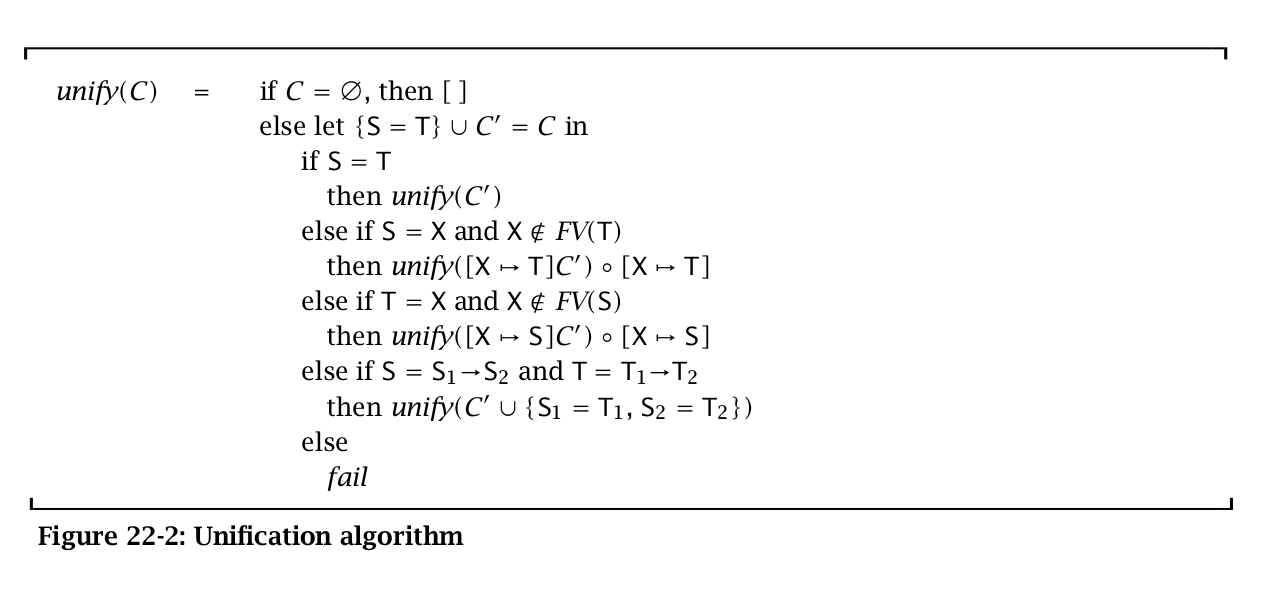
\includegraphics[width=\textwidth]{../hmunification.png}
    \caption{Unification algorithm}
    \label{hm-uni-algo}
  \end{figure}
  Note that the solution is not guaranteed to be unique. It may depend on the order of constraint solving.

  The type of $t$ under the principle unifier is called its \emph{principal type}.

  It's also possible to make type reconstruction incremental.



\section{Ch23: Universal Types}
\subsection{Elements}
  \label{systemf}
  On top of~\ref{simtyp}, see page~\pageref{simtyp}.
  Often called ``System F''.

\paragraph{Terms}
  Use $X$ as type variable, $T$ is a metavariable for types and may contain $X$.

  \begin{align*}
    t \quad ::= \quad
      & x \tag{var} \\
      & \lamt{x}{T}{t} \tag{abs} \\
      & \app{t}{t} \\
      & \lam{X}{t} \tag{type abstraction}\\
      & \tapp{t}{T} \tag{type instantiation}\\
  \end{align*}

\paragraph{Values}
  \begin{align*}
    v \quad ::= \quad
      & \lamt{x}{T}{t} \tag{abstraction} \\
      & \lam{X}{T} \tag{type abstraction}\\
  \end{align*}

\paragraph{Types}
  \begin{align*}
    T \quad::=\quad & T\to T \tag{function type} \\
      & X \tag{type variable}\\
      & \uquant{X}{T} \tag{universal type}\\
  \end{align*}

\paragraph{Contexts}
  \begin{align*}
    \Gamma \quad ::= \quad & \ldots \tag{empty, variable binding} \\
      & \Gamma, \, X \tag{type variable} \\
  \end{align*}

\paragraph{Semantics}
  \begin{align*}
      & \ldots \tag{E-APP1, E-APP2, E-APPABS} \\
      & \inference
        {t \to t_1}
        {t [T] \to t_1 [T]}
        \tag{E-TAPP}\\
      & (\lam{X}{T})\,  [T] \to [X\mapsto T]T
        \tag{E-TAPPABS}\\
  \end{align*}

\paragraph{Typing}
  \begin{align*}
    & \ldots \tag{T-VAR, T-ABS, T-APP} \\
    & \inference
      {\Gamma, X\vdash t : T}
      {\lam{X}{T} : \uquant{X}{T}}
      \tag{T-TABS}\\
    & \inference
      {\Gamma\vdash t : \uquant{X}{T}}
      {\Gamma\vdash \tapp{t}{T} : [X\mapsto T] T}
      \tag{T-TAPP} \\
  \end{align*}

\subsection{Concepts}
  \begin{itemize}
    \item Polymorphism: parametric (generically typed), ad-hoc (e.g. type case \verb|instanceof|), subtyping.
    \item System F originally was discovered as logic in proof theory.
    \item Church boolean e.g. $\lamt{x}{X}{\lamt{y}{X}{x}}$ has type $\uquant{X}{X\to X\to X}$.
    \item General type reconstruction to System F is undecidable.
      Partial reconstruction when type instantiation parameters can be left out
      is also undecidable.
    \item One approach to the above problem is partial type construction.
      1) Partial type inference with first-class existential types is present
      in ML as with the \verb|datatype| keyword.
      2) Local type inference supports subtyping and impredicative polymorphism
      is present in Scala.
      3) Greedy type inference is used in variable proof checkers.
    \item Another approach is to use a restricted fragment of System F.
      In ML polymorphic terms could only be constructed in let-in expressions.
      Only monotype (types without quantifiers) could appear in the lhs of a type abstraction.
      Rank-2 polymorphism restricts the depth of universally quantified type variables, and is another approach.

    \item Naive semantics for system F requires passing types around, which may introduce significant runtime costs. Thus type erasure semantics is introduced.

    \item System F is impredicative in that quantifiers in it could range over
      domains which the quantifier tries to define, as in $\uquant{X}{X\to X}$
      is a type but $X$ ranges over types. In ML polymorphism is predicative.
  \end{itemize}

\subsection{Examples}
\paragraph{Encoding pairs}
  $T_1$/$T_2$ stands the type for the first/second component.
  $X_3$ is a function transforming the two arguments into an output.
\begin{alignat*}{4}
  \mathrm{Pair} &\quad&=&\quad& \uquant{X_1}{\uquant{X_2}{\uquant{X_3}{(X_1\to X_2\to X_3) \to X_3}}}
  \\
  \mathrm{Pair}~T_1~T_2 &&=&& \uquant{X_3}{(T_1\to T_2\to X_3) \to X_3}
  \\
  \mathrm{mkPair}~t_1~t_2 &&=&& \lam{X}{\lam{Y}{
    \lamt{x}{X}{\lamt{y}{Y}{
      (\lam{X_3}{\lamt{f}{X\to Y\to X_3}{p~x~y}})
    }}
  }}
  \\
  \mathrm{mkPair} &&:&& \uquant{X}{\uquant{Y}{X \to Y \to \mathrm{Pair}~X~Y}}
  \\
  \mathrm{fst} &&=&& \lam{X}{\lam{Y}{
    \lamt{p}{\mathrm{Pair~X~Y}}{p~[X]~(\lamt{x}{X}{\lamt{y}{Y}{x}})}
  }}
\end{alignat*}

\paragraph{Church number encoding}
  Intuitively, we want $c_n = \underbrace{S~(S~(\ldots~(S}_{\text{A total of $n$ $S$'s}}Z)\ldots))$.
\begin{alignat*}{4}
  \mathrm{nat} &\quad&=&\quad& \uquant{X}{(X\to X)\to X \to X}
  \\
  Z &&=&& \lam{X}{
    \lamt{s}{X\to X}{\lamt{z}{X}{z}}
  }
  \\
  Z &&:&& \mathrm{nat}
  \\
  \mathrm{S} &&=&& \lamt{n}{\mathrm{nat}}{
    \lam{X}{
      \lamt{s}{X\to X}{\lamt{z}{X}{s~(n~[X]~s~z)}}
    }
  }
  \\
  S &&:&& \mathrm{nat}\to\mathrm{nat}
\end{alignat*}

\section{Ch24: Existential Types}
\subsection{Elements}
  On top of System F (section \ref{systemf}, page \pageref{systemf}).
  Only differences are listed. Diverges from TAPL book.

\paragraph{Terms}
  Packing simply choose a type and substitute it for an abstract type variable $X$.
  In packing, $T$ must be an existential type.
  \begin{align*}
    t \quad ::= \quad & \ldots \\
      & \epack{t}{T} \tag{packing} \\
      & \elet{X}{x}{t}{t} \tag{unpacking}
  \end{align*}

\paragraph{Values}
  $\{T, t\}$ has type $\equant{X}{T_1}$,
  when the type obtained by instatiating $X$ with $T$ in $T_1$ is the type of $t$.
  \begin{align*}
    v \quad ::= \quad & \ldots \\
      & \epack{v}{T}\\
  \end{align*}

\paragraph{Types}
  \begin{align*}
    T \quad ::= \quad & \ldots \\
      & \equant{X}{T} \tag{existential type} \\
  \end{align*}

\paragraph{Semantics}
  \begin{align*}
    & \elet{X}{x}{}
  \end{align*}

\paragraph{Typing}
  \begin{align*}
    & \ldots \\
    & \inference
      {\typjud{t}{[X\to T_1] T}}
      {\typjudp{\epack{t}{\equant{X}{T}}}{\equant{X}{T}}}
      \tag{T-PACK} \\
    & \inference
      {\typjud{t}{\equant{X}{T}},&
       \Gamma, X, x : T \vdash t_1 : T_1
      }{
        \typjudp{\elet{X}{x}{t}{t_1}}{T_1}
      }
      \tag{T-UNPACK}
  \end{align*}
% TODO

\subsection{Concepts}
  \begin{itemize}
    \item Two interpretations to existential types exist.
      The logical one, and the operational one which pairs a type with a term.
    \item Hiding the actual type for $\equant{X}{t}$ means restricting
      the applicable operations on data with the abstract type $X$.
    \item Existential types are often used to implement modules to hide actual
      type implementation, or ADTs (on page 369).
      An abstract data type consists of its name, the concrete representation, and exported operations on it.
      There is some boundary; in the boundary the concrete representation is visible and manipulatable;
      but outside the boundary, values of ADT are viewed abstractly, for which only those exported operations apply.
      ADTs achieve \emph{representational independence}, and improves robustness as well as maintainability in practice.
    \item Encapsulation in OOP can also be thought of as existential types.
      Depending on whether variants / operations is more often altered, objects or ADTs is preferred.
    \item In fact, existential types and universal types are dual -- like in logic $\uquant{x}{(p(x) \to Q)}$ is equivalent to $(\equant{x}{p(x)}) \to Q$
  \end{itemize}



\section{Ch26: Bounded Quantification}
\subsection{Elements}
  Basically on top of System F, but incorporating $\lambda_{<:}$ in a different way.
\begin{itemize}
  \item Replace $X$ with $X<:T$ in term definition, value definition, type definition, context definition and evaluation.
  \item The only nontrivial modification occurs in typing rules.
\end{itemize}

\paragraph{Terms}
  \begin{align*}
    t \quad ::= \quad & \ldots \tag{var, abs, app}\\
      & \lam{X<:T}{T} \tag{type abstraction}\\
      & \tapp{t}{T} \tag{type instantiation}\\
  \end{align*}

\paragraph{Values}
  \begin{align*}
    v \quad ::= \quad & \ldots \tag{abstraction} \\
      & \lam{X <: T}{T} \tag{bounded type abstraction}\\
  \end{align*}

\paragraph{Types}
  \begin{align*}
    T \quad::= \quad & T \to T \tag{function type} \\
      & X \tag{type variable}\\
      & \uquant{X<:T}{T} \tag{bounded universal type}
  \end{align*}

\paragraph{Contexts}
  \begin{align*}
    \Gamma \quad ::= \quad & \ldots \tag{empty, variable binding} \\
      & \Gamma, \, X <: T \tag{bounded type variable} \\
  \end{align*}

\paragraph{Semantics}
  \begin{align*}
      & \ldots \tag{E-APP1, E-APP2, E-APPABS, E-TAPP} \\
      & (\lam{X<:T}{T})\,  [T] \to [X\mapsto T]T
        \tag{E-TAPPABS}\\
  \end{align*}

\paragraph{Typing - part 1}
  Basically the same as in System F.
  \begin{align*}
    & \ldots \tag{T-VAR, T-ABS, T-APP} \\
    & \inference
      {\Gamma, X<:T\vdash t : T_1}
      {\lam{X<:T}{T_1} : \uquant{X<:T}{T_1}}
      \tag{T-TABS}\\
    & \inference
      {\Gamma\vdash t : \uquant{X<:T}{T_1}, \Gamma \vdash T_2 <: T}
      {\Gamma\vdash \tapp{t}{T_2} : [X\mapsto T_2] T_1}
      \tag{T-TAPP} \\
  \end{align*}

\paragraph{Typing - part 2}
  Subtyping for bounded universal types.
  Note that all judgements $T_1 <: T_2$ now need to be contexted i.e. $\Gamma\vdash T_1 <: T_2$.
  \begin{align*}
    & \ldots \tag{S-REFL, S-TRANS, S-TOP, S-ARROW} \\
    & \inference{X <: T \in \Gamma}{\Gamma\vdash X <: T}
      \tag{S-TVAR} \\
    & \inference
      {\Gamma, X<:T \vdash T_1 <: T_2}
      {\Gamma\vdash \uquant{X<:T}{T_1}\; <: \;\uquant{X<:T}{T_2}}
      \tag{S-ALL (kernel)} \\
    & \inference
      {\Gamma \vdash S_1 <: S_2, & \Gamma, X <: S_1 \vdash T_1 <: T_2}
      {\Gamma\vdash \uquant{X<:S_2}{T_1} \;<:\; \uquant{X<:S_1}{T_2}}
      \tag{S-ALL (full)} \\
  \end{align*}
  The S-ALL rule has two variants: kernel and full.
  The latter is more expressive, but the former is more practical.

\subsection{Concepts}
  \begin{itemize}
    \item Unbounded quantification is achieved with bounding by $\top$ type.
    \item Quantifiable type variables introduce a scoping problem for type terms in $\Gamma$ e.g. $\Gamma = X <: \{val : \mathrm{nat}, next : X\}$. By default we assume a type variable to be in scope after its occurrence so that no free type variables are allowed in a type term. When a type term may appear in its own definition, the system is called F-bounded quantification.
    \item Quantified universal types can be seen as mapping a collections of types onto its range.
  \end{itemize}

\subsection{Examples}
\paragraph{Encoding pairs}
  This time a pair type has to be annotated with its component types, because no free type variables are allowed.
\begin{alignat*}{4}
  \mathrm{Pair}~T_1~T_2 &\quad&=&\quad&
    \uquant{X<:T_1}{\uquant{Y<:T_2}{\uquant{Z<:Top}{(X\to Y\to Z) \to Z}}}
  \\
  \mathrm{mkPair}~T_1~T_2 &&=&&
    \lamt{x}{T_1}{\lamt{y}{T_2}{
      (\lam{Z<:\top}{\lamt{f}{X\to Y\to Z}{f~x~y}})
    }}
\end{alignat*}
  Without special handling it is possible to derive
\[
  \inference
    {\Gamma\vdash S_1<:S_2,& \Gamma\vdash T_1<:T_2}
    {\mathrm{Pair}~S_1~T_1 \quad<:\quad \mathrm{Pair}~S_2~T_2}
\]



\section{Ch29: Type Operators and Kinding}
\subsection{Elements}
  Based on $\lambda_{\to}$, called $\lambda_{\omega}$.

\paragraph{Kinds}
  \begin{align*}
    K \quad::=\quad & * \tag{proper type}\\
      K\Rightarrow K \tag{type operator}
  \end{align*}

\paragraph{Kinding}
  \begin{align*}
    & \inference
      {X :: K \in \Gamma}
      {\Gamma\vdash X :: K}
      \tag{K-TVAR}
    \\
    & \inference
      {\Gamma\vdash T_1 :: *,
      & \Gamma\vdash T_2 :: *}
      {\Gamma\vdash T_1 \to T_2 :: *}
      \tag{K-ARROW}
    \\
    & \inference
      {\Gamma, X :: K_1 \vdash T_2 :: K_2}
      {\Gamma\vdash \lamk{X}{K_1}{T_2}\;::\;K_1 \Rightarrow K_2}
      \tag{K-ABS}
    \\
    & \inference
      {\Gamma\vdash T_1 :: K_1 \Rightarrow K_2,
      & \Gamma\vdash T_2 :: K_1}
      {\Gamma\vdash T_1 T_2 :: K_2}
      \tag{K-APP}
  \end{align*}


\subsection{Concepts}
  \begin{itemize}
    \item ``Kinds are built from a single atomic kind written $*$''.
      Types with kind $*$ are called \emph{proper types}. Only well-formed types are proper types, e.g. $(\mathrm{Nat}~\mathrm{Nat})$ is ill-formed.
    \item Distinctions: The universal type $\uquant{X}{X\to X}$,
      for example $\mathrm{id} = \lam{X}{\lamt{x}{X}{x}}$, is a type with kind $*$,
      and it produced a term $\mathrm{id}_{X}$ for any type.
    \item Distinctions: The type constructor $\lam{X}{X}$,
      for example $\mathrm{some} = \lam{X}{X}$, is a type constructor with kind $* \Rightarrow *$,
      and it produced a type $\mathrm{some}~T$ for any type $T$.
    \item Definitional equivalence makes type operators like Haskell \texttt{type}s instead of \texttt{data}s or \texttt{newtype}s.
    \item Type expressions with kinds like $(* \Rightarrow *)\Rightarrow *$ are called \emph{higher-order type operators}.
    \item For Haskell, \texttt{Maybe} is a type (operator) with kind $*\Rightarrow *$.
        \texttt{JustA} (essentially \texttt{Just} but restrict the argument type to \texttt{A}) is a term with type $A\to \text{\texttt{Maybe}} A$.
        Also, \texttt{fmapAB} is a term with type $\lamk{F}{*\Rightarrow *}{ (A \to B) \to (F\, A\to F\, B) }$.
  \end{itemize}

\section{Ch30: Higher-Order Polymorphism}
\subsection{Elements}
  Based on $\lambda_{\omega}$ and System F, called F$_{\omega}$.

\paragraph{Types}
  \begin{align*}
    T \quad::=\quad & \ldots \tag{function type, type variable} \\
      & \uquant{X::K}{T} \tag{universal type}\\
      & \lamk{X}{K}{T} \tag{operator abstraction}\\
      & T~T \tag{operation application}
  \end{align*}

\paragraph{Kinding}
  \begin{align*}
    & \ldots \tag{K-TVAR, K-ABS, K-APP, K-ARROW}\\
    & \inference
      {\Gamma, X::K \vdash T :: *}
      {\Gamma\vdash (\uquant{X::K}{T}) :: *}
  \end{align*}

\subsection{Concepts}
  \begin{itemize}
    \item Both $\lambda_{\to}$ and System F are contained in F$_\omega$.
      By restricting the kinds allowed F$_n, n\in\mathbb{N}$ can be allowed.
      $\lambda_{\to}$ is F$_1$, while System F is F$_2$.
    \item Abstraction $\lamt{x}{T}{t}$ are terms, and can be seen as terms $\mapsto$ terms, like in \verb|func abs(int) int|.
    \item Type abstraction $\lamk{X}{K}{t}$ are terms, and can be seen as types $\mapsto$ terms, like in \verb|func<T> compare(T, T) int|.
    \item Type operators $\lamk{X}{K}{T}$ are types, and can be seen as types $\mapsto$ types, like in \verb|type<T> list|.
    \item Dependent types e.g. $\Pi n:\mathbb{N}\, .\;\mathbb{N}\to \mathrm{NatList}~n \to \mathrm{NatList}~(S~n)$ are types,
      an can be seen as terms $\mapsto$ types, like in C an ad hoc manner: \verb|int[n]|.
      They are closed related to verification, yet makes type checking intractable as a cost of the expressiveness.
    \item Bounded quantification are partial mappings (type $\mapsto$ term), like partial functions (term $\mapsto$ term).
      Constrained operators like in pseudo-Haskell
      \footnote{Haskell does not impose typeclass constraints on operator
      parameters -- the constraint is imposed when defining instances thus to
      be finer-grained.}
      \verb|data (Eq a) => Set a| are partial mappings (types $\mapsto$ types).
    \item Subtyping is not an element in the lambda cube.
      When combined with $\lambda_{\to}$ it yields trivial $\lambda_{<:}$.
      When combined with (System) F it yields bounded quantification.
  \end{itemize}



\section{Higher-Order Subtyping}
\subsection{Elements}
  Incorporating subtyping into F$_{\omega}$.

\paragraph{Kinding}
  \begin{align*}
    \inference
      {X <: T \in \Gamma,
      &\Gamma\vdash T :: K}
      {\Gamma\vdash X :: K}
      \tag{K-TVAR}
  \end{align*}

\paragraph{Subtyping}
  TODO

\subsection{Concepts}
  \begin{itemize}
    \item While it is possible to speficy $X::K$ and $X<:T$ at the same time,
      we must have $T :: K$ and the former can be left out.
  \end{itemize}

\end{document}

